\chapter{The hydrogen bond: the water dimer}
\label{sec:hydrogen-bond}
\index{Hydrogen bond}
\index{Water dimer}
\index{Intermolecular interactions}
\checkedwith{9.5.3-dev}{6dd630422}
\eccexample{Examples > General Chemistry > Intermolecular interactions}
\helppage{density-map}

\helppage{electron-density-views}

The hydrogen bond is usually drawn as a dotted line between a hydrogen atom and an oxygen or nitrogen atom of another molecule. This chapter gives the teacher pictures and numbers to show a class what that line stands for, all taken from two stored calculations of the General Chemistry example set: the water dimer, the smallest case of the bond, and the single water molecule. Each section takes one sign of the bond that students meet in a course, namely the energy that holds the pair together, the short distance between the molecules and the longer O--H bond of the donor, the lower and stronger O--H stretch in the infrared spectrum, and the electron density between the molecules, and names the ECCE panel that shows it and the chemical point it makes.

\section*{This requires}
Nothing beyond ECCE: the calculations are in the General Chemistry example set.

\section{Background}
This section gives the chemistry that the pictures in the rest of the chapter are read against. In O--H$\cdots$O the donor O--H group gives up a little electron density to the region between H and the acceptor oxygen. The attraction is mostly electrostatic: the positive end of one O--H dipole points at the negative region of the other molecule. In the water dimer the donor O--H points almost straight at the acceptor oxygen, and the acceptor's two hydrogens lie out of the plane of the bond.

A hydrogen bond between neutral molecules is far weaker than a covalent bond and several times stronger than the attraction between molecules of similar size without one. That is enough to give water its high boiling point and ice its open structure.

\section{The calculation}
The topic \menu{Intermolecular interactions} has two calculations made for this chapter, the water dimer \emph{h2o\_dimer} and the single molecule \emph{h2o\_monomer}. Both were optimised and their vibrations calculated with the same method, so their energies, structures and spectra can be compared directly.

\section{Procedure}
The steps show where in ECCE each number and picture of this chapter comes from; the sections that follow take them in the same order.
\begin{enumerate}
	\item In the Organizer, choose \menu{File > Open Example Calculations}, pick \menu{General Chemistry} and click \menu{OK}.
	\item In \menu{Examples > Intermolecular interactions}, select \emph{h2o\_dimer} and \emph{h2o\_monomer} and compare their total energies in the Organizer's table, or with \menu{Tools > Energy Calculator...}: dimer minus twice the monomer.
	\item Open \emph{h2o\_dimer} in the Viewer. With \menu{Measure} (Chapter~\ref{ch:first-calculation}), measure the distances O1--O4, H2--O4 and O1--H2, and the angle O1--H2--O4. Measure O--H in \emph{h2o\_monomer} too.
	\item Open \menu{Properties > Vibrational spectra > Vibrational Frequencies} in both and compare the O--H stretches above 3000~cm$^{-1}$, with their IR intensities.
	\item In the dimer, click \menu{Density Map}, choose the plane \menu{Through three atoms A, B, C} with O1, H2 and O4, and \menu{Show: Total density}. Click \menu{Density Profile} for the same density along the line from O1 to O4.
	\item Open \menu{Properties > Orbitals > Surfaces} and choose \menu{NCI}.
\end{enumerate}
\index{Energy Calculator}\index{Measure}\index{NCI}

\section{Interaction energy}
The first question for a class is whether the two molecules hold together at all, and how strongly. The dimer is \SI{26}{kJ.mol^{-1}} lower in energy than two separate molecules ($-152.862864$ against $2\times-76.426490$~hartree, the unit in which ECCE lists these energies; one hartree is \SI{2625.5}{kJ.mol^{-1}}). That is the energy it takes to pull the pair apart, the strength of this one hydrogen bond. It is about ten times $RT$ at room temperature (\SI{2.5}{kJ.mol^{-1}}), the typical energy that molecules exchange in collisions, because the positive end of the donor's O--H dipole sits right against the negative region of the acceptor oxygen. Hence a hydrogen bond survives many collisions before it breaks, which is why the molecules of liquid water stay held by their neighbours, while the bond is still weak enough to break and form again all the time.

\section{Geometry}
The bond also shows in the structure, measured with \menu{Measure}. O1--O4 is \SI{2.90}{\angstrom} and H2--O4 \SI{1.93}{\angstrom}, well inside the sum of the van der Waals radii of H and O (about \SI{2.7}{\angstrom}), the distance at which an H atom and an O atom of two molecules touch without any bond between them. The angle O1--H2--O4 is \ang{172.6}, nearly linear. The donor's O1--H2 bond is \SI{0.971}{\angstrom}, \SI{0.008}{\angstrom} longer than O--H in the single molecule (\SI{0.963}{\angstrom}).

The short H2--O4 distance shows that the molecules are pulled closer together than two molecules merely in contact, because H2 is attracted to O4, and the longer O1--H2 shows that this attraction weakens the donor's own bond, because it draws some of the density of that bond towards O4. Hence the hydrogen bond can be seen in the structure alone, and the weaker donor bond is what the infrared spectrum picks up next.

\section{Infrared spectrum}
The infrared spectrum is where a hydrogen bond is most often seen in a laboratory, and the \menu{Vibrational Frequencies} panel shows the calculated spectrum. The single molecule has its two O--H stretches at 3782 and 3888~cm$^{-1}$. In the dimer the stretch of the bonded O--H is at 3668~cm$^{-1}$, \SI{114}{cm^{-1}} lower, with an IR intensity of 315~km/mol against 4 and 44~km/mol in the single molecule. The intensity says how strongly a band absorbs infrared light, so the band of the bonded O--H is seven times as strong as the stronger O--H band of the single molecule. The other three stretches of the dimer, at 3780, 3858 and 3880~cm$^{-1}$, stay close to those of the free molecule.

The lower frequency follows from the structure, since the longer, weaker O1--H2 bond vibrates more slowly, and only the stretch of the bonded O--H shifts, which shows that the effect is confined to the bond that points at the acceptor. A low and strong O--H band, broad in a measured spectrum, is how a hydrogen bond is recognised in the laboratory.
\index{Infrared spectrum!hydrogen bond}\index{Red shift}

\section{Electron density}
The \menu{Density Map} and \menu{Density Profile} panels show where the electrons are between the two molecules, which is the way to ask what the dotted line of the textbook stands for. In the plane of the bond (figure~\ref{fig:hb-density}) the inner contours of the total density close around each molecule separately, and only the outer, low levels enclose both, with a narrow waist between H2 and O4, so the dimer remains two molecules held close together.

\begin{figure}[htbp]
	\centering
	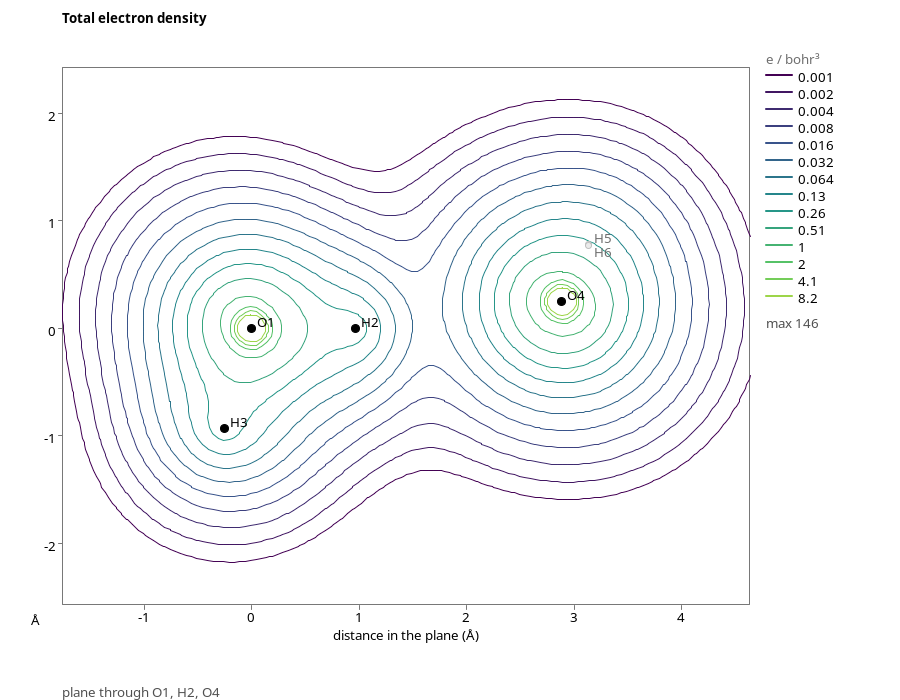
\includegraphics[width=0.8\linewidth]{hydrogen-bond/total-density.ecce-9.5.3-dev.png}
	\caption{Total electron density of the water dimer in the plane through O1, H2 and O4 (\menu{Density Map}). The contour levels double from 0.001~e/bohr$^3$ (0.001, 0.002, 0.004, \ldots), so each ring inward has twice the density of the one outside it. Only the outermost rings enclose both molecules.}
	\label{fig:hb-density}
\end{figure}

The \menu{Density Profile} along the line from O1 to O4, which passes almost through H2, puts numbers on the waist of the map (figure~\ref{fig:hb-profile}). The density is in electrons per cubic bohr (one bohr is \SI{0.529}{\angstrom}), on a logarithmic axis where each grid line is ten times the one below. Between H2 and O4 the density falls to a minimum of 0.0255~e/bohr$^3$, 0.66~\AA\ from H2. In the covalent O1--H2 bond it does not fall below 0.34~e/bohr$^3$, about thirteen times as much. The profile shows that the two molecules share very little electron density, because the hydrogen bond is mostly the electrostatic attraction of two separate molecules rather than an electron pair shared between them. Hence it is far weaker than a covalent bond, while the small density between H2 and O4 is still there, and the next view shows what kind of contact it is.
\index{Density Profile!hydrogen bond}

\begin{figure}[htbp]
	\centering
	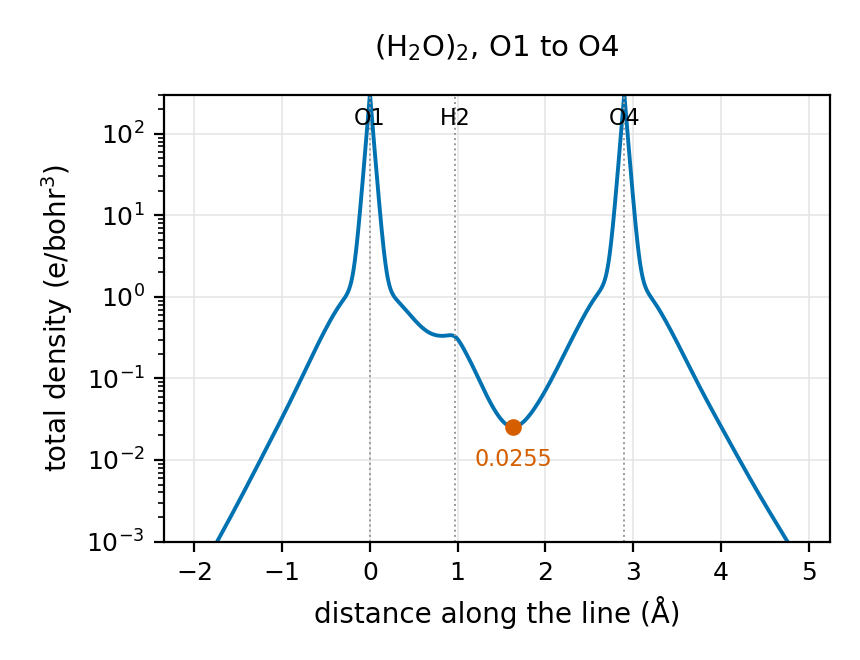
\includegraphics[width=0.6\linewidth]{hydrogen-bond/density-profiles.ecce-9.5.3-dev.png}
	\caption{Total electron density along the line from O1 to O4 of the water dimer (\menu{Density Profile}, logarithmic axis). The dot marks the lowest density between H2 and O4, 0.0255~e/bohr$^3$, about a thirteenth of the lowest density in the covalent O1--H2 bond.}
	\label{fig:hb-profile}
\end{figure}

\section{Non-covalent interactions}
The density map shows that there is a little density between H2 and O4, but not whether it pulls the molecules together or pushes them apart. The \menu{NCI} surface (non-covalent interactions) answers that, and it puts the hydrogen bond in one place in the picture (figure~\ref{fig:hb-nci}). ECCE draws the surface only where the electron density is low and changes slowly, which is true between molecules but not inside the covalent bonds or around the nuclei, so the bonds of each water molecule carry no surface and only the contacts between molecules do. It then colours the surface by the density there, with a sign that tells whether the density is gathered between two atoms or pushed apart: blue for attraction such as a hydrogen bond, green for weak contacts with little density, such as two molecules merely touching, and red for repulsion between atoms crowded too close. The colours run on one fixed scale for every calculation, so a blue surface in one molecule means the same as a blue surface in another.

In the water dimer the only surface is a small disc between H2 and O4, across the line between them, and it is blue. This shows that the density between the two molecules marks an attraction, because it is gathered between H2 and O4 rather than pushed apart. Hence the dotted line of the textbook has a place in the molecule, and the disc is where it crosses from one water molecule to the other.

\begin{figure}[htbp]
	\centering
	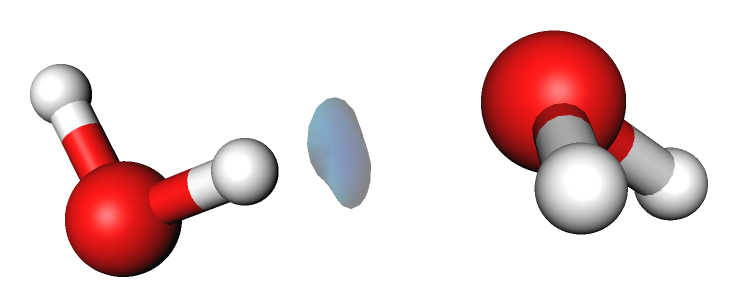
\includegraphics[width=0.6\linewidth]{hydrogen-bond/nci.ecce-9.5.3-dev.png}
	\caption{NCI surface of the water dimer (\menu{Properties > Orbitals > Surfaces}, \menu{NCI}), donor on the left and acceptor on the right. The only surface is the small disc between H2 and O4. Its colour tells the kind of contact on a fixed scale: blue attraction, as in a hydrogen bond; green a weak contact with little density; red repulsion. The disc is blue, an attraction; the surface is drawn partly transparent, which makes the blue look pale on a white background.}
	\label{fig:hb-nci}
\end{figure}

\section{In class}
Show the evidence in the order energy, distance, infrared, density: each is one more piece of evidence for the same bond, and the first three can be measured in a laboratory. The density map is the place to ask what the dotted line in the textbook stands for. It is not a line of electrons; the molecules stay separate, and what the map shows is a small extra amount of density between H and O on top of the overlap of two molecules. The NCI surface then puts the bond in one place, the blue disc between H2 and O4.

\section{History}
For a class, the origin of the idea shows that the hydrogen bond was proposed to explain the properties of water, the same properties the Background starts from. Latimer and Rodebush proposed in 1920 that a hydrogen atom held between two strongly electronegative atoms could bind them, to explain the properties of water and of hydrogen fluoride \cite{latimer1920}. Pauling made the hydrogen bond a part of structural chemistry in the 1930s, and it became central to biochemistry when it was shown to hold the base pairs of DNA and the helices and sheets of proteins together.
\index{Latimer, Wendell}\index{Rodebush, Worth}\index{Pauling, Linus}
